\subsection{13. Нормальная форма Хомского для КС-грамматик. Алгоритм приведения к нормальной форме Хомского.}

\Def КС-грамматика находится в нормальной форме Хомского, если все правила имеют такой и только такой вид:

\begin{enumerate}
    \item $A \rightarrow a \brackets{A \in N, \,\, a \in \Sigma}$;
    \item $A \rightarrow BC \brackets{B, C \in N; \,\, B, C \neq S}$;
    \item $S \rightarrow \varepsilon$.
\end{enumerate}


\Statement Любую КС-грамматику можно привести к нормальной форме Хомского с помощью алгоритма, который состоит из следующих шагов:

\begin{enumerate}
    \item Удаление непорождающих символов
    \item Удаление недостижимых символов
    \item Удаление смешанных правил $D \rightarrow aBc$
    \item Удаление длинных правил $A \rightarrow A_1 A_2 A_3 A_4$
    \item Удаление $\varepsilon$-порождающих символов
    \item Обработка пустого слова
    \item Удаление унарных (одиночных) правил $A \rightarrow B$
\end{enumerate}

\begin{itemize}
    \item[1-2.] После удаления непорождающих и недостижимых символов будет получена эквивалентная грамматика. Подробное доказательство этого есть в вопросе 12. Обозначим полученную грамматику за $G_2$.

    \item[3.] Для удаления смешанных правил сделаем замену правила вида $A \rightarrow d B c E f$ на правила следующего вида:
    $A \rightarrow D B C E F$, 
    $D \rightarrow d$, 
    $C \rightarrow c$, 
    $F \rightarrow f$.

Обозначим полученную грамматику за $G_3$. Покажем, что $w \in L \brackets{G_2} \Leftrightarrow w \in L \brackets{G_3}$. В основе доказательства лежит идея, что в дереве вывода нетерминальные символы можно выводить в любом порядке.

$\Rightarrow$
\begin{center}
    $A \vdash_1 dBcEf \vdash dw_B c w_E f$ $\brackets{G_2}$
    
    $A \vdash DBCEF \vdash dBcEf \vdash d w_B c w_E f$ $\brackets{G_3}$ 
\end{center}

$\Leftarrow$ Если в дереве вывода встречается $A \vdash DBCEF$, то раскрываем в первую очередь правила вида $D \rightarrow d$, а потом повторяем те же действия что в грамматике $G_2$ 

    \item[4.] Удалим длинные правила вида $B \rightarrow A_1 A_2 \dots A_n$ с помощью замены на правила следующего вида:

\begin{center}
    $B \rightarrow A_1 B_1 \qquad B_1 \rightarrow A_2 B_2 \qquad B_2 \rightarrow A_3 B_3 \qquad \ldots \qquad B_{n - 1} \rightarrow A_{n - 1} A_n$
\end{center}

Обозначим полученную грамматику за $G_4$. Покажем, что $w \in L \brackets{G_3} \Leftrightarrow w \in \brackets{G_4}$.

$\Rightarrow$ Пусть $w \in L \brackets{G_3}$. Тогда $S \vdash \varphi B \psi \vdash_1 \varphi A_1 A_2 \dots A_n \psi \vdash w$. Посмотрим, что происходит в $G_4$:
\begin{center}
    $S \vdash \varphi B \psi \vdash \varphi A_1 B_1 \psi \vdash \varphi A_1 A_2 B_2 \psi \vdash \dots \vdash \varphi A_1 A_2 \dots A_{n - 2} B_{n - 1} \psi \vdash \varphi A_1 \dots A_n \psi \vdash w$
\end{center}

$\Leftarrow$ Пусть $w \in L \brackets{G_4}$. Рассмотрим вывод $S \vdash w$. Возможны два варианта:

\begin{enumerate}
    \item $B_k$ не встречается на пути вывода. Тогда слово выводимо и в $G_4$, и в $G_3$;
    \item $B_k$ встречается на пути вывода. Тогда встречаются и все нетерминалы вида $B_1$, $\dots$, $B_{n - 1}$ по построению правил. Доказательство корректности аналогично доказательству в другую сторону.
\end{enumerate}

    \item[5.] Теперь остались правила вида:
\begin{center}
    $A \rightarrow a \qquad A \rightarrow BC \qquad A \rightarrow B \qquad A \rightarrow \varepsilon$
\end{center}

% \begin{enumerate}
%     \item $A \rightarrow a$;
%     \item $A \rightarrow BC$;
%     \item $A \rightarrow B$;
%     \item $S \rightarrow \varepsilon$.
% \end{enumerate}

Будем удалять $\varepsilon$ правила:
\begin{enumerate}
    \item Если $A \rightarrow BC$ и $C \vdash \varepsilon$, то добавим $A \rightarrow B$
    \item Если $A \rightarrow BC$ и $B \vdash \varepsilon$, то добавим $A \rightarrow C$
\end{enumerate}

Затем просто удаляем правила $A \rightarrow \varepsilon$. Получили грамматику $G_5$. Покажем корректность, то есть $w \in L(G_4) \Leftrightarrow w \in L(G_5)$ и $w \neq \varepsilon$.
\begin{figure}[h!]
        \centering
        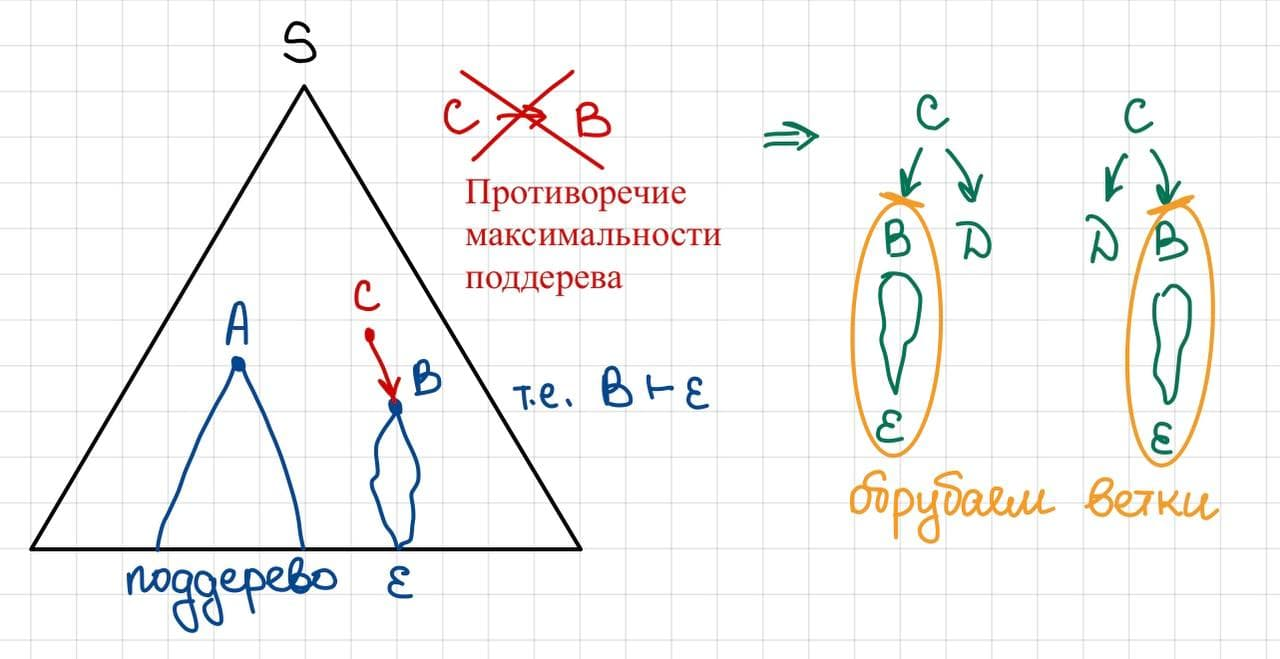
\includegraphics[scale=0.43]{images/tree.jpg}
        \label{fig:first}
\end{figure}

$\blacktriangle\Rightarrow$ Пусть $w \in L(G_4)$. Выделим поддеревья максимальной мощности из которых выводится $\varepsilon$ в дереве вывода $w$. Рассмотрим корень такого поддерева. Он не мог быть получен по правилу вида $C \rightarrow B$, так как тогда $C \vdash B \vdash \varepsilon$ и $C$ можно было бы включить в это поддерево, что противоречило бы максимальности. Поэтому корень $B$ был получен по правилу $C \rightarrow BD$ или $C \rightarrow DB$ (без ограничения общности рассмотрим первое). Тогда в $G_4$: $C \vdash_1 BD \vdash \varepsilon u = u$, а в $G_5$: $C \vdash_1 D \vdash u$, то есть ничего не поменялось $\Rightarrow w \in L(G_5)$

$\Leftarrow$ Пусть $w \in L(G_5)$. Рассмотрим правила вида $C \rightarrow D$ в дереве вывода $w$ в $G_5$, которых не было в $G_4$. Значит в $G_4$ было одно из правил $C \rightarrow BD, C\rightarrow DB$ и $B \vdash \varepsilon \Rightarrow w \in L(G_4) \blacksquare$

    \item[6.]Если $S \vdash \varepsilon$, то построим грамматику $G_6$ следующим образом:
\begin{enumerate}
    \item $S'$ — новый стартовый нетерминал;
    \item $S' \rightarrow S$ — новое правило;
    \item Если $S \vdash \varepsilon$, то $S' \rightarrow \varepsilon$ — новое правило.
\end{enumerate}

Данная грамматика будет эквивалентной. Этим шагом мы еще и частично приблизились ко второму пункту в определении НФ Хомского (не зацикливаемся на старте)

\item[7.] Рассмотрим последовательности правил:

\begin{center}
    $B \rightarrow B_1 \rightarrow B_2 \rightarrow \dots \rightarrow B_n \rightarrow CD$
    
    $B \rightarrow B_1 \rightarrow B_2 \rightarrow \dots \rightarrow B_n \rightarrow a$
\end{center}

Удалим унарные одиночные правила, заменим последовательности правил на $B \rightarrow CD$ и $B \rightarrow a$ соответственно (транзитивное замыкание). Обозначим полученную грамматику за $G_7$.

Покажем, что $L(G_6) = L(G_7)$. (= док-ву удаления $\varepsilon$-переходов в автомате).

$\Leftarrow$ Для всех правил вида $B \rightarrow a$ или $B \rightarrow CD$ верно, что $B \vdash_{G_6} a$, $B \vdash_{G_6} CD$. Никаких новых выводов добавлено не было, тем самым $L \brackets{G_7} \subseteq L \brackets{G_6}$.

$\Rightarrow$ Покажем, что $B \vdash_{G_6} w \Rightarrow B \vdash_{G_7} w$ индукцией по длине вывода.

\textbf{База.} Вывод за один шаг: $B \vdash_{G_6, 1} w \Longrightarrow \brackets{B \rightarrow w} \in P_{G_6}, w \in \Sigma \Longrightarrow \brackets{B \rightarrow w} \in P_{G_7} \Longrightarrow B \vdash_{G_7,1} w$.

\textbf{Переход.} Добавленное правило имеет вид $B \rightarrow C_1 \dots C_n$, где $n \in \{  1, 2\}$, $B \rightarrow C_1 \dots C_n \vdash_{G_6} w_1 \dots w_n$, по предположению индукции $C_i \vdash_{G_7} w_i$.

Пусть $n = 2$. Тогда правило имеет вид $B \rightarrow CD$, $B \vdash_{G_7} CD \vdash_{G_7} w_1 w_2$.

Пусть $n = 1$. Тогда вывод начинается с правила $B \rightarrow C_1$. Рассмотрим первое правило вывода, не являющееся одиночным. Тогда:

\begin{enumerate}
    \item $B \vdash C_1 \vdash C_2 \vdash \dots \vdash C_m \vdash a$, $a \in \Sigma$, тогда по построению существует правило $B \rightarrow a$, $B \vdash_{G_7} a$;
    \item $B \vdash C_1 \vdash C_2 \vdash \dots \vdash CD \vdash w_1 w_2$. По построению существует правило $B \rightarrow CD$, по предположению индукции $B \vdash_{G_7} CD \vdash w_1 w_2$.
\end{enumerate}

Построенная грамматика $G_7$ — грамматика в нормальной форме Хомского.

\end{itemize}